\documentclass[a4paper, 12pt]{article}
\usepackage[utf8]{inputenc}
\usepackage[lmargin=3cm, tmargin=3cm, rmargin=2cm, bmargin=2cm]{geometry}
\usepackage[onehalfspacing]{setspace}
\usepackage[T1]{fontenc}
\usepackage[brazil]{babel}

\usepackage{wasysym}%male and female

\usepackage{graphicx, graphics, xcolor, comment, enumerate, multirow, multicol, indentfirst}

\usepackage{amsmath, amsthm, amsfonts, amssymb, dsfont, mathtools}
\everymath{\displaystyle} 

\usepackage{blindtext}

\usepackage[round]{natbib}
\bibliographystyle{apalike}

%Code packages:
\usepackage{listings}
\usepackage{xcolor}

%New colors defined below
\definecolor{codegreen}{rgb}{0,0.6,0}
\definecolor{codegray}{rgb}{0.5,0.5,0.5}
\definecolor{codepurple}{rgb}{0.58,0,0.82}
\definecolor{backcolour}{rgb}{0.95,0.95,0.92}

%Code listing style named "mystyle"
\lstdefinestyle{mystyle}{
  backgroundcolor=\color{backcolour},   commentstyle=\color{codegreen},
  keywordstyle=\color{magenta},
  numberstyle=\tiny\color{codegray},
  stringstyle=\color{codepurple},
  basicstyle=\ttfamily\footnotesize,
  breakatwhitespace=false,         
  breaklines=true,                 
  captionpos=b,                    
  keepspaces=true,                 
  numbers=left,                    
  numbersep=5pt,                  
  showspaces=false,                
  showstringspaces=false,
  showtabs=false,                  
  tabsize=2
}

%"mystyle" code listing set
\lstset{style=mystyle}

\title{Projeto 1: Administração Florestal}
\author{
  Gabriel Mota Lima\\
  \texttt{11794870}
  \and
  Herberth Luan Vieira Oliveira\\
  \texttt{12559110}
  \and
  Mateus Queiroz de Souza Daniel\\
  \texttt{11294552}
  \and
  Victor Viana de Oliveira Matos\\
  \texttt{11810821}
  \and
  Vinícius da Costa Collaço\\
  \texttt{11811012}
}


\begin{document}

\maketitle

\section{Introdução}

A sustentabilidade nunca foi tão discutida como é atualmente, são reuniões com líderes políticos e leis criadas para que cada vez se tenham a conscientização da utilização dos recursos dados da natureza de maneira mais responsável possível, sendo que são finitos.

Com isso em mente o uso de modelos matemáticos juntamente com o poder computacional ficaram mais procurados, visto que uma parte da matemática trabalha com resolução de problemas de máximos e mínimos e deste modo auxiliando diversas áreas para que façam os seus processos de maneira a não desperdiçar materiais que são utilizados nos processos, ou seja, otimização do uso. 

Nesse trabalho é apresentado modelo matemático dado um problema de plantio de árvores, o qual objetivo será o modelo deixar o teu plantio sustentável e otimizando o retorno para plantador.

\subsection{Situação-problema e conceitos}
O contexto que será aplicado modelo matemático é de uma área, onde encontra-se um vetor inicial x de formação de árvores de variadas alturas n, as quais terão um crescimento em determinado período. Após o crescimento será feita a colheita e replantio delas. O problema consiste em realizar um modelo matemático que tenha um corte sustentável e que economicamente se tenha um retorno sustentável ótimo para o proprietário.

Alguns conceitos se fazem importante explicitá-los para que o modelo matemático fique mais entendível, seriam: corte sustentável e retorno sustentável ótimo.

Corte sustentável, conforme Anton Rorres, pode-se definir o corte sustentável quando após o processo de crescimento e colheita a configuração final seja igual a tua inicial, ou seja, retornar ao vetor inicial x. A Figura 1 abaixo mostra de maneira mais lúcida o termo de corte sustentável:




\begin{center}
    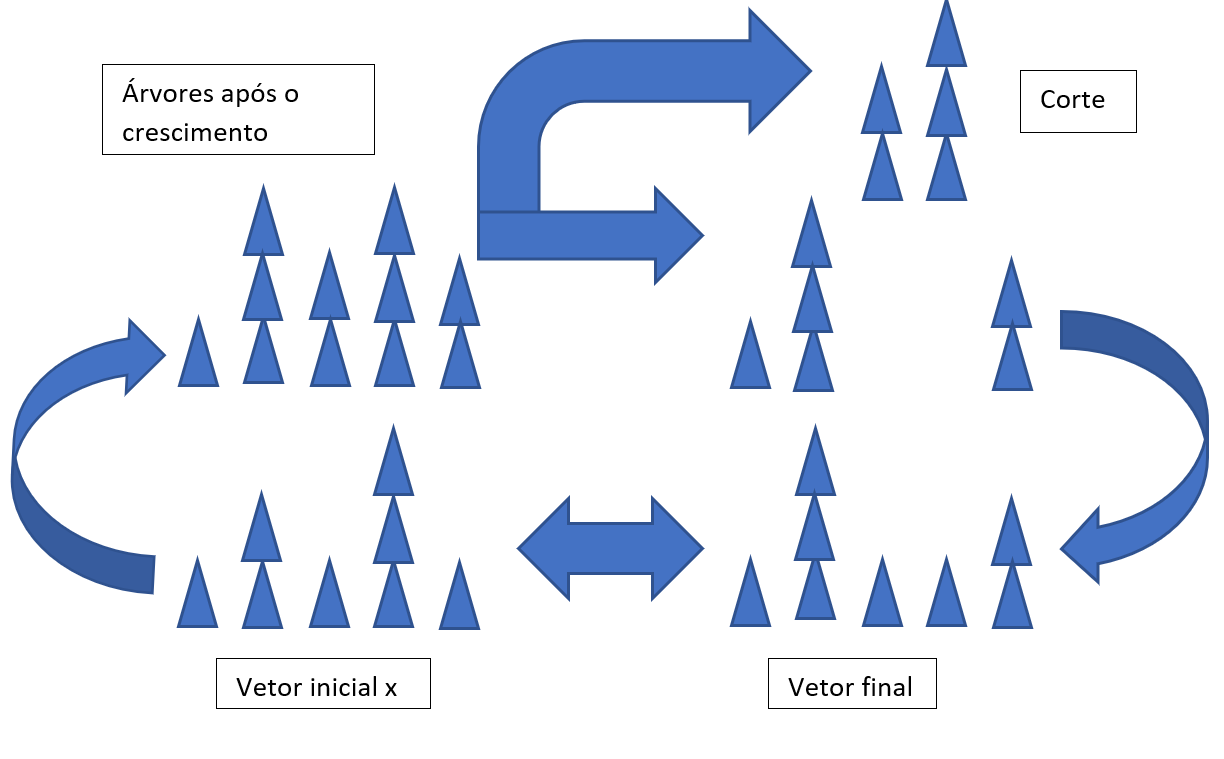
\includegraphics[width=13cm]{colheita-sustentavel.PNG}
    
    Figura 1: Colheita Sustentável
\end{center}

Retorno Sustentável Ótimo é definido por um teorema, de acordo com Anton Torres, o rendimento é obtido cortando todas as árvores de uma classe de altura específica e nenhuma árvore de qualquer outra classe. Portanto, esse conceito será a base para o modelo matemático consiga otimizar o corte economicamente para o plantador.

\subsection{Modelo Matemático}

Por definição, modelo é uma representação da realidade que acaba sendo simplificada e idealizada, portanto, algumas restrições que serão colocadas para que seja aplicável e atendido a situação-problema.

O primeiro momento a organização das árvores é a partir de classes avaliando pela altura, sendo que a primeira classe será a muda a qual foi passado que não há custos e nem receita para essa classe e que dada classe n não há mais crescimento. Os valores econômicos são função das respectivas alturas.

Dentro do modelo há algumas restrições que seguem:

•	cada árvore no teu período de crescimento só consegue crescer de uma classe, exceto àquelas que estejam na classe n, pois essa se mantém;

•	nenhum uma árvore morre nenhum dos processos;

•	os preços são fixados;

•	as taxas de crescimento são fixadas para cada classe


\section{Equações que definem uma colheita sustentável}

Para termos uma colheita sustentável, a configuração final da floresta( após o corte e plantio das mudas) deve ser igual à configuração inicial (floresta antes do crescimento).
Como, no nosso modelo, o número  de árvores é constante e igual a s, podemos descrever a configuração inicial da floresta como sendo um vetor coluna $\mathrm{x}$, chamado de vetor de não cortadas. $\;\;\;$
$\mathrm{x} = 
  \begin{bmatrix}
  x_1 \\
  x_2 \\
  \vdots  \\
  x_n 
\end{bmatrix}\;$
onde $\mathrm{x_i}$ representa a quantidade de árvores da classe i (sendo que as árvores são classificadas pelo intervalo de altura a que pertencem e a classe 1 corresponde a mudas sem valor comercial) e $\mathrm{s=\sum\limits_{i=1}^{n}x_i}$.
 
Após cada colheita, as árvores passam por um período de crescimento, onde uma fração $\mathrm{g_i}$ das árvores de cada classe i sobe para a classe i+1, obtendo-se assim a configuração pré-corte.
 
O número de árvores em cada classe i, na configuração pré-corte, é igual à soma entre o número de árvores da classe i-1 que cresceram ($\mathrm{g_{i-1}\cdot x_{i-1}}$) e o número de árvores da classe i que não cresceram ($\mathrm{(1-g_{i})\cdot x_i}$), com exceção da classe 1, onde restarão apenas as mudas que não cresceram, e da classe n onde apenas serão somadas as árvores que cresceram da classe n-1. Assim obtemos o vetor da configuração pré-corte:

$\;\;\;$
$$\mathrm{Z} = 
  \begin{bmatrix}
  x_1 \cdot (1-g_1) \\
  x_2 \cdot (1-g_2) + x_1 \cdot g_1\\
  \vdots  \\
  x_n + x_{n-1} \cdot g_{n-1}
\end{bmatrix}\;$$ 
 
No entanto, convém escrever o vetor pré-corte como o o produto entre uma "matriz de crescimento" (G) e o vetor x, sendo que: $\:$
$\mathrm{G} = \begin{bmatrix}
  1-g_1 & 0 & 0 & & \cdots & 0 \\
  g_1 & 1-g_2 & 0 & & \cdots & 0 \\
  0 & g_2 & 1-g_3 & & \cdots & 0 \\
  \vdots  & \vdots  & \vdots & & \vdots &\vdots \\
  0 & 0 & 0 & \cdots & 1-g_{n-1} & 0 \\
  0 & 0 & 0 & \cdots & g_{n-1} & 1
 \end{bmatrix}$
 
 O vetor de árvores cortadas é dado por $\mathrm{y}$. $\;\;\;$
$\mathrm{y} = 
  \begin{bmatrix}
  y_1 \\
  y_2 \\
  \vdots  \\
  y_n 
\end{bmatrix}\;$ onde cada $\mathrm{y_i}$representa a quantidade de árvores cortadas na classe i.
 
Para que haja uma colheita sustentável,  será plantado um número de mudas igual ao número de árvores retiradas.
 
Assim,sabemos que o vetor reposição a ser somado ao vetor pré-corte ($\mathrm{G \cdot x}$) e ao vetor -y para se obter o vetor x deve possuir um valor igual à soma do número de árvores cortadas em todas as classes (exceto da classe 1, composta por mudas sem valor comercial) em sua primeira linha:
 
$\mathrm{F} =
  \begin{bmatrix}
  \sum\limits_{i=2}^{n}y_i \\  0 \\
  \vdots  \\
  0 
  \end{bmatrix}$ 
 
Portanto podemos definir uma matriz de reposição $\mathrm{R}$, de ordem n, como sendo a matriz que faz real a igualdade $F=R\cdot \mathrm{y}$.
$\;$
$\mathrm{R} = 
 \begin{bmatrix}
  1 & 1 & \cdots & 1 \\
  0 & 0 & \cdots & 0 \\
  \vdots  & \vdots  &  & \vdots  \\
  0 & 0 & \cdots & 0 
 \end{bmatrix}$

Com todas as variáveis do modelo podemos escrever matematicamente a equação que caracteriza uma política de corte sustentável.
 
$$\mathrm{Gx} - \mathrm{y} + \mathrm{Ry} = \mathrm{x} $$ 
 
ou também reescrita como 
\begin{equation}\label{colheita_sustentavel_matricial}
    \mathrm{(I - R)y = (G-I)x} 
\end{equation}
 
\textbf{Colocando y em função de x tem-se:} $\mathrm{y = (I - R)^{-1}(G-I)x}$

onde $\mathrm{G}$ e $\mathrm {R}$ e a matriz identidade $\mathrm {I}$ possuem dimensões $n \times n$, $\: \mathrm {x}$ e $\mathrm {y}$ são matrizes coluna com dimensão $n \times 1$, sendo $n$ o número de classes de árvores da floresta.

como $y_1 > 0$ representaria o corte de mudas, sem valor econômico e reposição por novas mudas, então deduzimos que:
\begin{equation}\label{y1_zero}
    y_1 = 0
\end{equation}
 
Com o resultado de (\ref{y1_zero}), equação (\ref{colheita_sustentavel_matricial}) pode ser escrita como um conjunto de equações da seguinte maneira:
\begin{equation}\label{igualdades_sustentaveis}
\begin {matrix}
    y_2 + y_3 + \cdots + y_n & = & g_1 x_1 \\ 
    y_2 & = &g_1 x_1 - g_2 x_2 \\
    y_3 & = &g_2 x_2 - g_3 x_3 \\
    & \vdots &  \\
    y_{n-1} & = &g_{n-2} x_{n-2} - g_{n-1} x_{n-1} \\
    y_n & = & g_{n-1} x_{n-1}
    \end {matrix}
\end{equation}
 
nesse sistema temos que a primeira equação é a soma das demais, pois os valores de $g_n, x_n\: $e $\:y_n$ são positivos, então as equações em (\ref{igualdades_sustentaveis}) exigem que:
 
\begin{equation}\label{desigualdades_sustentaveis}
    g_1x_1 \geq g_2x_2 \geq \cdots \geq g_{n-1}x_{n-1} \geq 0
\end{equation}
 
Portanto, para termos uma colheita sustentável, $\mathrm{x} \: e \: \mathrm {y} \: $devem satisfazer a equação (\ref{colheita_sustentavel_matricial}) e as entradas do vetor coluna $\mathrm {x}$ devem satisfazer à inequação (\ref{desigualdades_sustentaveis}), para que a floresta tenha uma configuração tal qual permita um corte sustentável.
 
Com o resultado obtido podemos criar um algoritimo que dado as entradas: n (número de classes da floresta), X (vetor de configuração da floresta, tamanho n), G (vetor de crescimento da floresta, tamanho n-1) e Y (vetor colheita, tamanho n), ele nos retorna True se a colheita é sustentável, ou False se a colheita não é sustentável.\newline

\begin{lstlisting} [language=Python, caption=Funcão para definir se um corte é ou não sustentável, label=listing_EhSustentavel]
def EhSustentavel(n,X,G,Y): 
  #Valores de entrada, n valor inteiro; X,G e Y, vetores
  import numpy as np
  
  #Tratando as entradas e criando a matriz identidade
  I = np.identity(n) #Matriz identidade n x n
  G_n_mais1 = G.copy()
  G_n_mais1.append(0) #vetor G com n+1 para gerar a matriz G n x n
  G = np.array(G)
  Gmc = np.atleast_2d(G).T #transforma o vetor G em matriz coluna
  X = np.array(X)
  Xmc = np.atleast_2d(X).T #transforma o vetor X em matriz coluna
  Y = np.array(Y)
  Ymc = np.atleast_2d(Y).T #transforma o vetor Y em matriz coluna

  #Matriz G n x n vinha do vertor G n-1
  GMatriz = I-(G_n_mais1*I)
  for i in range (n-1):
    GMatriz [i+1,i]=Gmc[i,0]
  GMatriz [n-1,n-1] = 1

  #Matriz R
  R = np.zeros((n,n))
  for i in range (n):
    R[0,i] = 1

  #Vetor GX para comparacao
  GX = [] 
  for i in range (n-2,-1,-1):
    GX.append(G[i]*X[i])
  GX = np.array (GX) #array com valores de g de n * x de n do ultimo para o primeiro
  
  #Operacoes colheita sustentavel para comparacao posterior
  valor1 =(I-R).dot(Ymc)
  valor2 = (GMatriz-I).dot(Xmc)


  #Condicoes Para Colheita sustentavel
  if Y[0] != 0: return False #Se o primeiro valor de Y for 0 retorna False
  elif GX[0] < 0: return False
  elif np.all(np.diff(GX) > 0) == False: return False # retorna False se nao for g1x1>g2x2>...
  elif (valor1.round()  == valor2.round()).all() == False: return False #Retorna falso se a floresta nao se manter igual apos a colheita
  else: return True
\end{lstlisting}

Com base em (\ref{y1_zero}) e (\ref{igualdades_sustentaveis}) podemos criar um algoritimo simples para retorna o vetor $\mathrm{y}$, que é o vetor da colheita sustentável dado uma certa configuração $\mathrm{x}$ da floresta e um crescimento $\mathrm{G}$:

\begin{lstlisting} [language=Python, caption=Retorna o vetor Y, label=listing_Retorno Y]
def ValoresY (g,x):
  y = [0]#primeiro valor sempre 0
  n = len(x)

  for i in range (1,n-1):
    y.append((g[i-1]*x[i-1])-(g[i]*x[i]))
    y[i]=round(y[i])#arrendondar os valores 
  y.append(g[-1]*x[-2])# yn = gn-1*xn-1
  y[-1]=round(y[-1])
  return y
\end{lstlisting}

\begin{center}
    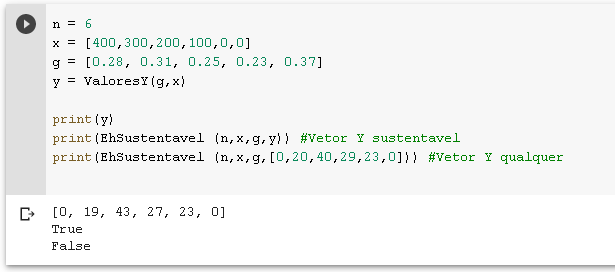
\includegraphics[width=13cm]{SaidaPrg.PNG}
    
    Figura 2: Saida de Teste das funções anteriores
\end{center}


\section{Modelando o problema em questão}
\subsection{Função objetivo}
O principal objetivo do modelo aqui proposto é maximizar o retorno financeiro da colheita, dadas as restrições que propiciam uma colheita sustentável e outras restrições práticas.

Sendo o retorno de cada colheita um somatório dos produtos entre a quantidade de árvores cortadas de cada classe e seus respectivos preços, tem-se que o retorno financeiro total de cada colheita é dado por (lembrando que $y_1=0$):

$$RT\ =\ p_2y_2+p_3y_3+...+p_ny_n$$

Então, usando-se as equações em (\ref{igualdades_sustentaveis}) tem-se que a função objetivo do modelo proposto é dada por:

\begin{equation}\label{funcao_objetivo}
    RT\ =\ p_2g_1x_1+\left(p_3-p_2\right)g_2x_2+...+\left(p_n-p_{n-1}\right)g_{n-1}x_{n-1}
\end{equation}

A função $RT$ é a função de \textbf{retorno sustentável} deve ser maximizada com relação às variaveis $x_1{,}\ x_2{,}\ ...\ {,}x_n$ para que se encontre o \textbf{retorno sustentável ótimo}.

\subsection{Restrições}

Uma das restrições que se pode estabelecer está relacionada com a capacidade total de plantio da floresta, isto é, a quantidade total de árvores plantadas não deve exceder a um determinado valor. No caso deste problema, considera-se que a quantidade de árvores no inicio do período de crescimento é sempre constante e igual a $s$, isto é:

\begin{equation}\label{restricao_somatorio}
x_1+x_2+...+x_n=s
\end{equation}
O conjunto de desigualdades apresentados em (\ref{desigualdades_sustentaveis}) são condições necessárias e suficientes para que a configuração estabelecidade pelo vetor $x$ permita que ocorra uma colheita sustentável. Portanto, (\ref{desigualdades_sustentaveis}) representa mais um conjunto de restrições do nosso modelo.

O último conjunto de restrições está associado ao fato de que o número de árvores em cada classe no inicio do período de crescimento não pode ser negativo, isto é:

\begin{equation}\label{restricao_positividade}
    x_1{,}\ x_2{,}\ ...\ {,}x_n\ge 0
\end{equation}

\subsection{O modelo}

Assim, dada a função objetivo (\ref{funcao_objetivo}) e as restrições (\ref{desigualdades_sustentaveis}), (\ref{restricao_somatorio}) e (\ref{restricao_positividade}) apresentadas acima pode-se modelar o problema da seguinte forma:


\begin{equation}\label{modelo_simples}
    \begin{cases}
    Max\ RT\ =\ p_2g_1x_1+\left(p_3-p_2\right)g_2x_2+...+\left(p_n-p_{n-1}\right)g_{n-1}x_{n-1}\\
    sujeito\ a:\\
    x_1+x_2+...+x_n=s\\
    g_1x_1\ge g_2x_2\ge \cdots \ge g_{n-1}x_{n-1}\ge 0\\
    x_1{,}\ x_2{,}\ ...\ {,}x_n\ge 0
    \end{cases}
\end{equation}

O modelo descrito em (\ref{modelo_simples}) é um problema de programação linear, pois tanto a função objetivo quanto as restrições são de grau 1 com respeito às variaveis $x_1{,}\ x_2{,}\ ...\ {,}x_n$.

\section{Encontrando o retorno sustentável ótimo}
\subsection{Teorema 1}
 
Para encontrar o retorno ótimo será considerado o seguinte teorema:

"O rendimento sustentável ótimo é obtido cortando todas as ávores de uma classe de altura específica e nenhuma árvore de qualquer outra classe" \citep{teorema_escrito_anton}.

\subsection{Função de retorno ótimo como implicação do Teorema 1}

Considerando que a classe $k$ é a única que tem as árvores completamente cortadas, então todos os $y_i$ $(i \ne k)$ devem ser iguais a zero, isto é:

\begin{equation}\label{yi_iguais_a_zero}
    y_2=y_3=...=y_{k-1}=y_{k+1}=...=y_n=0
\end{equation}

Somente $y_k \ne 0$.

Estamos considerando que a cada período de crescimento as ávores de uma determinada classe só podem crescer para a classe imediatamente superior. Se sempre cortarmos todas as árvores da classe $k$, então nunca haverá árvores nas classes superiores a $k$. E após o corte, também não haverá nenhuma árvore na classe $k$. Então tem-se:

\begin{equation}\label{xi_ge_k_zero}
    x_k=x_{k+1}=...=x_n=0
\end{equation}

Se substituirmos (\ref{yi_iguais_a_zero}) e (\ref{xi_ge_k_zero}) na equação (\ref{igualdades_sustentaveis}) chegamos ao seguinte resultado:

$$\begin{cases}
y_k=g_1x_1\\
0=g_1x_1-g_2x_2\\
0=g_2x_2-g_3x_3\\
 \vdots \\
0=g_{k-2}x_{k-2}-g_{k-1}x_{k-1}\\
y_k=g_{k-1}x_{k-1}
\end{cases}\ \Longrightarrow \ \begin{cases}
y_k=g_1x_1\\
g_1x_1=g_2x_2\\
g_2x_2=g_3x_3\\
\vdots \\
g_{k-2}x_{k-2}=g_{k-1}x_{k-1}\\
g_{k-1}x_{k-1}=y_k
\end{cases}$$\newline

Isto é: 
\begin{equation}\label{yk_gixi}
    y_k=g_1x_1=g_2x_2=...=g_{k-1}x_{k-1}
\end{equation}

A partir do resultado (\ref{yk_gixi}) acima, colocando todos os $x_i$ $(i \ne 1)$ em função de $x_1$, tem-se:

$$
x_2=\frac{g1\cdot x_1}{g_2}{,}\ \ x_3=\frac{g1\cdot x_1}{g_3}{,}\ ...\ {,}\ x_{k-1}=\frac{g_1\cdot x_1}{g_{k-1}}
$$

Substituindo as expressões acima na equação (\ref{restricao_somatorio}), pode-se isolar o valor de $x_1$:

$$
x_1+\frac{g1\cdot x_1}{g_2}+\frac{g1\cdot x_1}{g_3}+...\ +\frac{g_1\cdot x_1}{g_{k-1}}=s
$$
$$
x_1\cdot \left(1+\frac{g_1}{g_2}+\frac{g_1}{g_3}+...+\frac{g_1}{g_{k-1}}\right)=s
$$
$$
x_1=\frac{s}{1+\frac{g_1}{g_2}+\frac{g_1}{g_3}+...+\frac{g_1}{g_{k-1}}}
$$
\begin{equation}\label{x1_em_funcao_de_parametros}
    x_1=\frac{s}{g_1\cdot \left(\frac{1}{g_1}+\frac{1}{g_2}+\frac{1}{g_3}+...+\frac{1}{g_{k-1}}\right)}
\end{equation}

Como somente serão cortadas as árvores da classe $k$, então o retorno ótimo será dado pelo preço das árvores da classe $k$ (isto é $p_k$) multiplicado pela quantidade de árvores removidas ($y_k$). Então:

$$RT = p_k \cdot y_k$$

Pela relação (\ref{yk_gixi}), $y_k=g_1x_1$, então:

\begin{equation}\label{RT_pkg1x1}
    RT=p_k \cdot g_1 \cdot x_1
\end{equation}

Substituindo (\ref{x1_em_funcao_de_parametros}) na relação (\ref{RT_pkg1x1}) acima, tem-se:

$$
RT=p_k\cdot g_1\cdot \left[\frac{s}{g_1\cdot \left(\frac{1}{g_1}+\frac{1}{g_2}+\frac{1}{g_3}+...+\frac{1}{g_{k-1}}\right)}\right]
$$

Portanto, tem-se:
\begin{equation}\label{RT_teorema}
    RT_k=\frac{p_k\cdot s}{\frac{1}{g_1}+\frac{1}{g_2}+\frac{1}{g_3}+...+\frac{1}{g_{k-1}}}
\end{equation}

Desta forma, testa-se a função (\ref{RT_teorema}) para todos as classes de árvores. A classe $k$ que retornar o maior valor de $RT_k$ é a que deve ser completamente remotida.

\subsection{Valor do retorno ótimo}
Escrevendo matematicamente o resultado encontrado anteriormente:\newline

Definições:

$n$: quantidade de classes de altura para as árvores.

$s$: quantidade total de árvores no periodo de crescimento.

$\left\{p_2{,}\ p_3{,}\ ...\ {,}\ p_n\right\} $: preços das árvores em cada classe.

$\left\{g_1{,}\ g_2{,}\ ...\ {,}\ g_{n-1}\right\}$: parâmetros de crescimento das $n-1$ primeiras classes.\newline

Dadas as definições acima, o retorno sustentável ótimo pode ser escrito matematicamente como:
\begin{equation}\label{Ret_Maximo_RTk}
    Ret=Maximo\left\{\frac{p_k\cdot s}{\frac{1}{g_1}+\frac{1}{g_2}+\frac{1}{g_3}+...+\frac{1}{g_{k-1}}}\right\}, (k = 2, 3, ..., n)
\end{equation}

\subsection{Classe que será cortada}

A classe que será cortada é a classe $k$ ($k=2, 3, ..., n$) tal que $RT_k$ é máximo. 

\subsection{Algoritmo em Python para encontrar o retorno ótimo}

A relação demonstrada em (\ref{Ret_Maximo_RTk}) apresenta um algoritmo que demanda um processo de iteração. Pode-se fazer esta iteração em uma linguagem de programação. O código a seguir representa a definição da função \emph{retorno\_otimo} na linguagem Python (linguagem usada durante todo este trabalho), que tem como parâmetros g e p, que recebem como argumentos objetos Python do tipo \emph{list}, contendo respectivamente os parametros de crescimento e os preços das ávores de cada classe (com exceção de $g_n$ e $p_1$). Há também os parâmetros n e s, que recebem como argumentos, respectivamente, a quantidade de classes de alturas das árvores e a quantidade total de árvores no período de crescimento. A função itera por todos os valores de $k=2, 3, ..., n$ e calcula todos os valores de $RT_k$.\newline

\begin{lstlisting}[language=Python, caption=Função retorno\_otimo, label=listing_funcao_retorno_otimo]
def retorno_otimo(n, s, p, g):
  retornos = []
  for i in range(n-1): #se tem 6 classes, i itera entre [0,1,2,3,4]
    soma_inversos_g = 0 
    for j in range(i+1): # loop para calcular o denominador de RT_k
      soma_inversos_g = soma_inversos_g + 1/g[j]
    r = p[i]*s / soma_inversos_g # calcula RT_k para cada classe k
    retornos.append(round(r, 2)) # armazena os retornos para cada classe
  return (retornos, max(retornos), 2+retornos.index(max(retornos)))

\end{lstlisting}

A função acima retorna três objetos:\newline

\textbf{retornos}: lista contendo os todos os valores de $RT_k$ pra todos os valores de $k$ possíveis.

\textbf{max(retornos)}: função que retorna o valor numérico do maior retorno, isto é, retorna o maior valor de $RT_k$.

\textbf{2+retornos.index(max(retornos))}: índice da classe que será cortada. Soma-se 2 ao índice do maior retorno, pois a iteração é feita com base na lista de preços que começa em $p_2$, isto é, quando $k=2$ o indice do vetor retornos é $0$.

Assim, por meio da função acima, o retorno sustentável ótimo é conseguido através da segunda posição da \emph{tupla} retornada pela chamada da função. Por exemplo:

\begin{lstlisting}[language=Python, caption=Encontrando o retorno ótimo, label=listing_chamada_retorno_otimo]
_, Ret, classe_cortada = retorno_otimo(classes, s, precos, g)
\end{lstlisting}

A variável \emph{Ret} por ser a segunda posição na atribuição das variáveis irá armazenar o retorno ótimo. E por seguinte, a variável \emph{classe\_cortada} armazenará o número correspondente a classe que será cortada.
A chamada de função demonstrada na \emph{Listing \ref{listing_chamada_retorno_otimo}}, bem como a função escrita na \emph{Listing \ref{listing_funcao_retorno_otimo}} serão usados para resolver o exercício prático seguinte.

\section{Resolução de um problema prático}
É dado um problema com os seguintes valores para os parâmetros g, p e n:

$$g_1=0.28, g_2=0.31, g_3=0.25, g_4=0.23 e g_5=0.37$$
$$p_2=50, p_3=100, p_4=150, p_5=200, p_6=250$$
$$n=6$$

Dados estes valores, falta apenas o valor de $s$ para que possamos substituir na função da \emph{Listing \ref{listing_funcao_retorno_otimo}}  que retrata o algoritmo (\ref{Ret_Maximo_RTk}) e encontrar o retorno ótimo. Como todos os valores de $RT_k$ estão em função do parâmetro $s$, para que se encontre o maior valor de $RT_k$ não importa o valor de $s$. Então escolhemos um valor arbitrário para substituir na relação e testar no algoritmo em Python, neste caso $s=1000$.


\subsection{Resolução em Python usando o resultado do Teorema 1}

Foram criadas variáveis para armazenar os valores referidos acima, são elas:

\begin{lstlisting}[language=Python, caption=Definindo os valores das variáveis, label=listing_definindo_variaveis]
g = [0.28, 0.31, 0.25, 0.23, 0.37]
precos = [50, 100, 150, 200, 250]
classes = 6
s = 1000 #valor arbitrario
\end{lstlisting}

Em seguida chamamos a função \emph{retorno\_otimo} definina em \emph{Listing \ref{listing_funcao_retorno_otimo}}, e passamos a ela os argumentos definidos em \emph{Listing \ref{listing_definindo_variaveis}}. Armazena-se então os valores que esta função retorna nas seguintes variáveis:

\begin{lstlisting}[language=Python, caption=Chamando a função \emph{retorno\_otimo} e armazenando retornos, label=listing_chamada_retorno_otimo_2]
vetor_retornos, Ret, classe_cortada = retorno_otimo(classes,s,precos,g)
\end{lstlisting}

\subsubsection{Classe cortada}

Como retorno da função, será armazenado na variável \emph{classe\_cortada} o número correspondente a classe que será cortada completamente.

Observando pelo console do Python, tem-se que o valor da classe a ser cortada neste caso é a \textbf{classe 3}, como é retratado abaixo:

\begin{lstlisting}[language=Python, caption=Valor da variável \emph{classe\_cortada}, label=listing_console_classe_cortada]
>>> classe_cortada
3
\end{lstlisting}


\subsubsection{Retorno sustentável ótimo}

Do mesmo modo, verificando pelo console do Python o valor assumido pela variável $Ret$, conclui-se que o retorno ótimo para este exercício é de R\$14.711,00 (para $s=1000$ árvores), que é obtido ao se cortar todas as árvores da terceira classe.
\begin{lstlisting}[language=Python, caption=Valor da variável \emph{Ret}, label=listing_console_Ret]
>>> Ret
14711.86
\end{lstlisting}

\subsection{Resolução algébrica usando o resultado do Teorema 1}

Sendo $k = 2, 3, 4, 5, 6$, faz-se a iteração demandada pela relação (\ref{Ret_Maximo_RTk}) como se segue:

$$RT_2=\frac{p_2\cdot s}{\frac{1}{g_1}}=\frac{50s}{\frac{1}{0.28}}=14s$$
$$RT_3=\frac{p_3\cdot s}{\frac{1}{g_1}+\frac{1}{g_2}}=\frac{100s}{\frac{1}{0.28}+\frac{1}{0.31}}=14.711s$$
$$RT_4=\frac{p_4\cdot s}{\frac{1}{g_1}+\frac{1}{g_2}+\frac{1}{g_3}}=\frac{150s}{\frac{1}{0.28}+\frac{1}{0.31}+\frac{1}{0.25}}=13.892s$$
$$RT_5=\frac{p_5\cdot s}{\frac{1}{g_1}+\frac{1}{g_2}+\frac{1}{g_3}+\frac{1}{g_4}}=\frac{200s}{\frac{1}{0.28}+\frac{1}{0.31}+\frac{1}{0.25}+\frac{1}{0.23}}=13.205s$$
$$RT_6=\frac{p_6\cdot s}{\frac{1}{g_1}+\frac{1}{g_2}+\frac{1}{g_3}+\frac{1}{g_4}+\frac{1}{g_5}}=\frac{250s}{\frac{1}{0.28}+\frac{1}{0.31}+\frac{1}{0.25}+\frac{1}{0.23}+\frac{1}{0.37}}=14s$$

\subsubsection{Classe cortada}
 O maior valor de de $RT_k$ ocorre quando $k=3$, então é a classe 3 que deve ser cortada. Concordante com o resultado encontrado na seção anterior.
\subsubsection{Retorno sustentável ótimo}
Independentemente do número total de árvores $s$ na floresta, o retorno sustentável ótimo neste caso é $14.711s$ (maior valor de $RT_k$). Este valor é condizente com os R\$14.711,86 encontrados com a função $retorno\_otimo$ no Python, para $s=1000$.

\subsection{Resolução em Python pelo algoritmo Simplex}
Para uma análise comparativa com os resultados encontrados anteriormente, se utilizará aqui o método simplex que é um dos métodos mais importantes da área de programação linear \citep{livro_pesquisa_operacional}, e serve para se determinar a solução ótima em problemas de otimização linear, como é o caso do modelo proposto em (\ref{modelo_simples}).

\subsubsection{Preparação para a implementação}
A implementação do método simplex aqui será baseada na forma padrão retratada a seguir, que é o modelo aceito pelo método $scipy.optimize.linprog(method='simplex')$, da biblioteca Pyhon chamada $SciPy$ (\cite{simplex_scipy}).

\begin{center}
    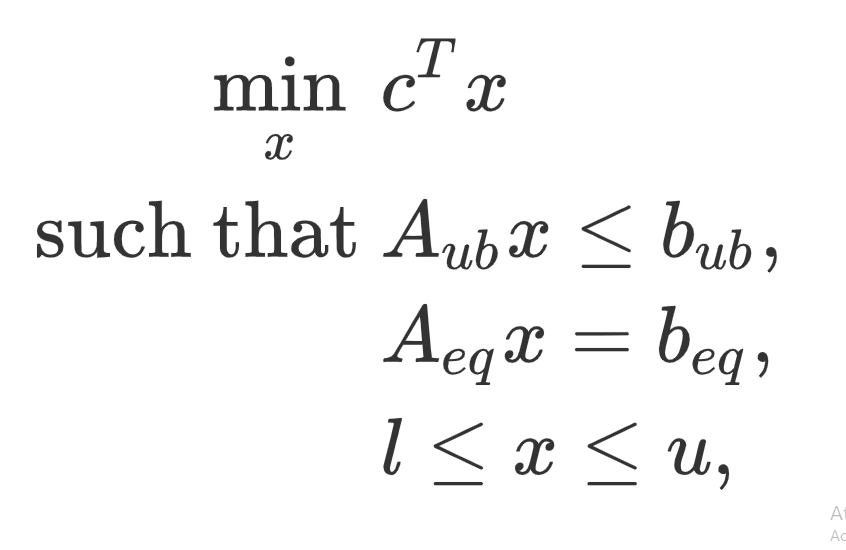
\includegraphics[width=5cm]{scipy-simplex-formato.PNG}
    
    Figura 2: Formato do problema de programação Linear aceito pela biblioteca
\end{center}

Por padrão, a biblioteca trabalha com valores não negativos para as variáveis de decisão $x_1, x_2, ..., x_n$. Então não será necessário definir as condições de não negatividade na programação em Python, que estão representadas na figura acima por $l\le x\le u$, e define limites infirior e superior para as variáveis de decisão.

Para que o modelo em (\ref{modelo_simples}) se adeque ao aceito pela biblioteca $SciPy$ devemos reescreve-lo. Este modelo pede que se maximize $RT$, então no modelo $SciPy$, devemos minimizar o inverso de $RT$ isto é: $min$ $(-1)\cdot RT$.

Além disso, nas restrições todas as inequações devem estar na forma $\mathrm{A_{\mathit{ub}}\mathrm{x\mathit{\le \mathrm{b\mathit{_{ub}}}}}}$ e igualdades na forma $\mathrm{A_{\mathit{eq}}\mathrm{x\mathit{= \mathrm{b\mathit{_{eq}}}}}}$.

Assim, fazendo as alterações necessárias em nosso modelo, considerando os valores de parâmentros de crescimento e preços dados e sendo s=1000, tem-se:

\begin{equation}\label{modelo_adequado_simplex}
    \begin{cases}
Min\ -RT\ =\ -14x_1-15.5x_2-12.5x_3-11.5x_4-18.5x_5-0x_6\\
sujeito\ a:\\
x_1+x_2+x_3+x_4+x_5+x_6=1000\\
-0.28x_1+0.31x_2\le 0\\
-0.31x_2+0.25x_3\le 0\\
-0.25x_3+0.23x_4\le 0\\
-0.23x_4+0.37x_5\le 0\\
x_1{,}\ x_2{,}\ x_3{,}\ x_4{,}\ x_5{,}\ x_6\ge 0
\end{cases}
\end{equation}

Colocando na forma matricial para que possamos escrever nosso programa tem-se:

\textbf{Função objetivo:}

$$ -RT=\begin{pmatrix}
-14&-15.5&-12.5&-11.5&-18.5&0
\end{pmatrix}\begin{pmatrix}
x_1\\
x_2\\
x_3\\
x_4\\
x_5\\
x_6
\end{pmatrix} $$\newline

\textbf{Restrições:} 

Desigualdade ($\mathrm{A_{\mathit{ub}}\mathrm{x\mathit{\le \mathrm{b\mathit{_{ub}}}}}}$):

$$\begin{pmatrix}
-0.28&0.31&0&0&0&0\\
0&-0.31&0.25&0&0&0\\
0&0&-0.25&0.23&0&0\\
0&0&0&-0.23&0.37&0
\end{pmatrix}\begin{pmatrix}
x_1\\
x_2\\
x_3\\
x_4\\
x_5\\
x_6
\end{pmatrix}\le \begin{pmatrix}
0\\
0\\
0\\
0
\end{pmatrix}$$

Igualdade ($\mathrm{A_{\mathit{eq}}\mathrm{x\mathit{= \mathrm{b\mathit{_{eq}}}}}}$):

$$\begin{pmatrix}
1&1&1&1&1&1
\end{pmatrix}\begin{pmatrix}
x_1\\
x_2\\
x_3\\
x_4\\
x_5\\
x_6
\end{pmatrix}=\left(1000\right)$$

As condições de não negatividade não foram inclusas pois como explicitado elas já são assumidas como padrão pela biblioteca usada.

\subsubsection{Implementação em Python}

Definindo as variáveis em Python de acordo com as matrizes acima tem-se:

\begin{lstlisting}[language=Python, caption=Simplex: definindo as matrizes, label=listing_simplex_definindo as matrizes]
s = 1000

negativo_RT = [-14, -15.5, -12.5, -11.5, -18.5, 0]

A_ub = [[-0.28,  0.31,     0,     0,    0, 0],
        [    0, -0.31,  0.25,     0,    0, 0],
        [    0,     0, -0.25,  0.23,    0, 0],
        [    0,     0,     0, -0.23, 0.37, 0]]
b_ub = [0,
        0,
        0,
        0]

A_eq = [[1, 1, 1, 1, 1, 1]]
b_eq = [s]
\end{lstlisting}

Agora, passando as variáveis definidas acima como argumento ao método $linprog$ da biblioteca $scipy.optimize$, armazena-se na variável $otimo$ os resultados da otimização realizada com o algoritimo simplex.

\begin{lstlisting}[language=Python, caption=Simplex: otimizando, label=listing_simplex_otimizando]
from scipy.optimize import linprog

otimo = linprog(c=negativo_RT, A_ub=A_ub, b_ub=b_ub, A_eq=A_eq, 
                b_eq=b_eq, method='Simplex')
\end{lstlisting}

\subsubsection{Retorno sustentável ótimo}

Agora a variável $otimo$ contém todos os resultados da otimização. Pode-se acessar o retorno ótimmo, por meio do comando $otimo.fun$, porém neste caso será retornado um valor negativo, pois trata-se do mínimo de $-RT$, que corresponde ao máximo de $+RT$, então basta que verifiquemos o valor de $-otimo.fun$. Observe:

\begin{lstlisting}[language=Python, caption=Simplex: retorno ótimo arredondando para 2 casas decimais, label=listing_simplex_retorno_otimo]
>>> -otimo.fun.round(2)
14711.86
\end{lstlisting}

Portanto o retorno sustentável ótimo é de R\$14.711,86 (quando $s=1000$), condizente com todos os resultados encontrados anteriormente.

\subsubsection{Configuração inicial da floresta que permite um corte sustentável}

Pode-se também, por meio da otimização realizada com o método simplex, acessar o conteúdo do vetor x tal que RT é máximo. Isto é, podemos acessar a configuração inicial da floresta que permite um corte sustentável ótimo (para $s=1000$):

\begin{lstlisting}[language=Python, caption=Simplex: vetor x, label=listing_simplex_vetor_x]
>>> otimo.x.round(0).tolist()
[525.0, 475.0, 0.0, 0.0, 0.0, 0.0]
\end{lstlisting}

Como pode-se verificar, neste caso a configuração inicial da floresta é tal que:

$$\mathrm{x}=\begin{pmatrix}
x_1\\
x_2\\
x_3\\
x_4\\
x_5\\
x_6
\end{pmatrix}=\begin{pmatrix}
525\\
475\\
0\\
0\\
0\\
0
\end{pmatrix}$$

Isto é:

\begin{equation}\label{valores_de_xi}
    x_1 = 525, x_2=475, x_3=0, x_4=0, x_5=0, x_6=0
\end{equation}

\section{Valor de $p_5$ para que seja a classe 5 a ser cortada}
\subsection{Resolução Algébrica}

Como verificado na resolução algébrica feita na seção 5.2, para os preços e parâmetros de crescimento dados, o retorno sustentável ótimo é obtido cortando-se todas as árvores da classe 3, dando um retorno de $RT_3=14.711s$.

Portanto, para que seja a classe 5 aquela a ser totalmente removida, o valor de $RT_5$ deve ser maior que $14.711s$, se $RT_5=RT_3$ seriamos indiferentes entre cortar totalmente somente as árvores da classe 3 ou somente as da classe 5.

Assim, matematicamente deve-se ter:

$$RT_5>14.711s$$
$$\frac{p_5\cdot s}{\frac{1}{g_1}+\frac{1}{g_2}+\frac{1}{g_3}+\frac{1}{g_4}}>14.711s$$
$$\frac{p_5}{\frac{1}{0.28}+\frac{1}{0.31}+\frac{1}{0.25}+\frac{1}{0.23}}>14.711$$
$$p_5>222.81$$

Desta forma, o preço das árvores da classe 5 para que seja esta a ser cortada deve ser maior que R\$222,81.

\textbf{Então $p_5$ deve ser pelo menos igual a R\$222,82}.

\subsection{Simulação em Python}
Neste caso basta fazer testes sucessivos, nos quais se aumenta progrssivamente o valor de $p_5$ até que $RT_5$ seja o maior valor dentre todos os $RT_k$. Ao se incrementar $p_5$ desta forma, \textbf{o primeiro valor de $p_5$ que faz $RT_5$ ser máximo é o preço necessário para que a quinta classe seja a que vamos retirar completamente para termos o retorno sustentável ótimo.}

A implementação em Python do processo iterativo descrito é representada a seguir e utiliza a função $retorno\_otimo$ definida em \emph{Listing \ref{listing_funcao_retorno_otimo}}, que realiza o processo descrito em (\ref{Ret_Maximo_RTk}). Aproveita-se também a lista $precos$ definida em \emph{Listing \ref{listing_definindo_variaveis}}, de modo que $precos[3]$ representa $p_5$.

\begin{lstlisting}[language=Python, caption=Encontrando $p_5$ tal que $RT_5$ é máximo, label=listing_encontrando_p5]
s = 1000
classe_cortada = -1
while classe_cortada != 5: #testa-se ate que classe_cortada == 5
  precos[3] = precos[3] + 0.001 
  __, Ret, classe_cortada = retorno_otimo(classes, s, precos, g)
\end{lstlisting}

No algoritmo acima, incrementa-se o valor de $p_5$ em $0.001$ a cada passo até que $classe\_cortada$ seja igual a $5$. Assim, o último valor de $precos[3]$ registrado na memória é o valor de $p_5$ que faz $RT_5$ ser máximo. 


\begin{lstlisting}[language=Python, caption=Valor de $p_5$ tal que $classe\_cortada$ é 5, label=listing_valor_de_p5]
>>> round(precos[3], 2)
222.82
\end{lstlisting}

\textbf{Portanto o valor de $p_5$ para que seja a quinta classe a ser cortada é: R\$222,82}. Valor este que é condizente com a solução algébrica demonstrada anteriormente.\newline

Na \emph{Listing \ref{listing_encontrando_p5}} a variável $s$ está definida com o valor $1000$, porém alterando-se o valor de $s$ para qualquer outro valor como $s=10, 100, 1000000$, o valor encontrado de $precos[3]$ é sempre o mesmo e igual a R\$222,82.



\section{relação entre $p_2$, $p_3$, $p_4$, $p_5$ e $p_6$ para que qualquer que seja a classe cortada, teremos retorno sustentável ótimo}

Para que tenhamos um retorno sustentável ótimo qualquer que seja a classe a ser cortada, sendo $k=2,3,4,5,6$, o retorno oferecido ao se cortar qualquer uma das classes deve ser o mesmo, então:

\begin{equation}\label{RT2_RT3_RT4_RT5_RT6}
    RT_2=RT_3=RT_4=RT_5=RT_6
\end{equation}

Como queremos encontrar a razão entre os preços, podemos estabelecer arbitrariamente o valor de um deles. Então por conveniência, seja $p_2=1$ o preço das árvores da classe 2 que dê retorno ótimo.

Cortando a classe $k$, o retorno ótimo é dado por (\ref{RT_teorema}). Assim, para $k=2$ e $p_2=1$, tem-se:

\begin{equation}\label{RT2_028s}
    RT_2=\frac{p_2\cdot s}{\frac{1}{g_1}}=\frac{1\cdot s}{\frac{1}{0.28}}\therefore RT_2=0.28s
\end{equation}

Substituindo (\ref{RT2_028s}) em (\ref{RT2_RT3_RT4_RT5_RT6}):
$$ 0.28s=RT_3=RT_4=RT_5=RT_6 $$

Dados os valores de $g_1$, $g_2$, $g_3$, $g_4$ e $g_5$, temos então:

$$RT_3=\frac{p_3\cdot s}{\frac{1}{g_1}+\frac{1}{g_2}}\therefore 0.28s=\frac{p_3\cdot s}{\frac{1}{0.28}+\frac{1}{0.31}}\therefore p_3=1.9$$
$$RT_4=\frac{p_4\cdot s}{\frac{1}{g_1}+\frac{1}{g_2}+\frac{1}{g_3}}\therefore 0.28s=\frac{p_4\cdot s}{\frac{1}{0.28}+\frac{1}{0.31}+\frac{1}{0.25}}\therefore p_4=3.02$$
$$RT_5=\frac{p_5\cdot s}{\frac{1}{g_1}+\frac{1}{g_2}+\frac{1}{g_3}+\frac{1}{g_4}}\therefore 0.28s=\frac{p_5\cdot s}{\frac{1}{0.28}+\frac{1}{0.31}+\frac{1}{0.25}+\frac{1}{0.23}}\therefore p_5=4.24$$
$$RT_6=\frac{p_6\cdot s}{\frac{1}{g_1}+\frac{1}{g_2}+\frac{1}{g_3}+\frac{1}{g_4}+\frac{1}{g_5}}\therefore 0.28s=\frac{p_6\cdot s}{\frac{1}{0.28}+\frac{1}{0.31}+\frac{1}{0.25}+\frac{1}{0.23}+\frac{1}{0.37}}\therefore p_6=5$$

Isto é:

$$p_2=1, p_3=1.9, p_4=3.02, p_5=4.24, p_6=5$$

Então a razão entre os preços $p_2:p_3:p_4:p_5:p_6$ para que qualquer que seja a classe cortada dê retorno sustentável ótimo é:

$$1:1.9:3.02:4.24:5$$

\section{Quantidade de ávores removidas em cada colheita}

\subsection{Resolução algébrica}

A quantidade $r$ de árvores removidas é dada por:

$$r=y_2+y_3+...+y_n$$

Pela primeira equação do sistema (\ref{igualdades_sustentaveis}), tem-se que:
$$y_2 + y_3 + \cdots + y_n = g_1 x_1$$

Então:
\begin{equation}\label{r_g1x1}
r=g_1 \cdot x_1    
\end{equation}

Usando a expressão (\ref{x1_em_funcao_de_parametros}) de $x_1$ em função dos parâmetros $s$ e $g$, e substituindo na relação (\ref{r_g1x1}) acima, tem-se:

$$r=g_1\left[\frac{s}{g_1\left(\frac{1}{g_1}+\frac{1}{g_2}+...+\frac{1}{g_{k-1}}\right)}\right]$$

Por fim, a quantidade de árvores removidas pode ser dada por:

$$r=\frac{s}{\frac{1}{g_1}+\frac{1}{g_2}+...+\frac{1}{g_{k-1}}}$$

Sendo $k$ a classe que será completamente removida.

Para o exemplo prático iniciado na seção 5, a classe removida é a terceira, portanto $k=3$ na fórmula acima. Então para este problema, temos:

$$r=\frac{s}{\frac{1}{g_1}+\frac{1}{g_2}}=\frac{s}{\frac{1}{0.28}+\frac{1}{0.31}}\therefore r=0.147s$$

\textbf{Portanto para este exemplo, como $r=0.147s$, a quantidade de árvores removidas é sempre $14.7\%$ da quantidade total de árvores na floresta.}

Por exemplo, para o caso em que $s=1000$, a quantidade de árvores removidas em cada colheita é:

$$r=0.147 \cdot s=0.147 \cdot 1000$$
$$r=147$$

\subsection{Comparação com a resposta do algoritmo Simplex}

Apenas para efeito de comparação, usaremos aqui o valor de $x_1$ encontrado na seção 5 a partir da implementação do algoritmo simplex como parte da solução ótima (quando $s=1000$).

Por (\ref{valores_de_xi}) sabe-se que quando $s=1000$, $x_1=525$. Substituindo em (\ref{r_g1x1}), tem-se:

$$r=g_1 \cdot x_1  \therefore r=0.28 \cdot 525 $$
$$r = 147$$

Condizente com o resultado encontrado anteriormente.

\section{Verificando numericamente o resultado de otimalidade}
\subsection{Apresentação}

Como visto acima, para que o vetor x determine uma configuração da floresta que permita um corte sustentável, os valores de $x_i$ devem satisfazer as seguintes condições, que são condições necessárias e suficientes para que o objetivo de sustentabilidade seja atingido (além é claro do fato de que $x_i\ge 0$):

$$g_1x_1\ge g_2x_2\ge ...\ge g_{n-1}x_{n-1}\ge 0$$

Para o caso do problema em questão, deve-se ter:

\begin{equation}\label{experimento_desigualdades_sustentaveis}
    0.28x_1\ge 0.31x_2\ge 0.25x_3\ge 0.23x_4\ge 0.37x_5 \ge 0
\end{equation}

Assim, não é difícil encontrar configurações da floresta que permitam um corte sustentável. Por exemplo, se $s=1000$, a seguinte configuração permite um corte sustentável:

\begin{equation}\label{experimento_valores_xi_01}
    x_1=900, x_2=100, x_3=0, x_4=0, x_5=0, x_6=0
\end{equation}

Já que: 
$$0.28\cdot 900\ge 0.31\cdot 100\ge 0.25\cdot 0\ge 0.23\cdot 0\ge 0.37\cdot 0 \ge 0$$
$$252\ge 31\ge 0\ge 0\ge 0\ge 0$$

Levando-se em conta a função de retorno financeiro que já assume as condições de corte sustentável, istó é, a função de \textbf{retorno sustentável} vista em (\ref{funcao_objetivo}) e aplicando-a ao presente problema, tem-se que a função de retorno sustentável neste caso é dada por:

\begin{equation}\label{RT_experimento}
    RT=14x_1+15.5x_2+12.5x_3+11.5x_4+18.5x_5
\end{equation}

Substituindo os valores em (\ref{experimento_valores_xi_01}) tem-se:
$$RT=14\cdot 900+15.5\cdot 100+12.5\cdot 0+11.5\cdot 0+18.5\cdot 0$$
$$RT=\$ 14.150,00$$

Portanto fazendo um corte sustentável em uma floresta que tem a configuração vista em (\ref{experimento_valores_xi_01}) dá um retorno financeiro de R\$ 14.150,00, que não é o maior valor financeiro que pode ser obtido para uma floresta com 1000 árvores. Como visto na discussão sobre o retorno sustentável ótimo, o máximo retorno financeiro que pode ser obtido a partir de um corte sustentável em uma foresta com 1000 árvores é de R\$14.711,86. 

\subsection{Verificando o retorno sustentável para diferentes configurações de florestas}

Fazendo o procedimento anterior para algumas configurações de florestas que passam no teste (\ref{experimento_desigualdades_sustentaveis}), monta-se a seguinte tabela para uma floresta que comporta 1000 árvores:

$$\begin{array}{ | l | l | l | l | l | l | l | l | }
\hline
	Configuracao & x_1 & x_2 & x_3 & x_4 & x_5 & x_6 & RT \\ \hline
	1 & 350 & 300 & 200 & 100 & 50 & 0 & R\$ 14.125,00 \\ \hline
	2 & 400 & 300 & 200 & 100 & 0 & 0 & R\$ 13.900,00 \\ \hline
	3 & 400 & 350 & 200 & 50 & 0 & 0 & R\$ 14.100,00 \\ \hline
	4 & 450 & 350 & 200 & 0 & 0 & 0 & R\$ 14.225,00 \\ \hline
	5 & 450 & 400 & 150 & 0 & 0 & 0 & R\$ 14.375,00 \\ \hline
	6 & 500 & 450 & 50 & 0 & 0 & 0 & R\$ 14.600,00 \\ \hline
	7 & 510 & 460 & 30 & 0 & 0 & 0 & R\$ 14.645,00 \\ \hline
	\textbf{8 (ótimo)} & \textbf{526} & \textbf{474} & \textbf{0} & \textbf{0} & \textbf{0} & \textbf{0} & \textbf{R\$ 14.711,00} \\ \hline
	9 & 600 & 400 & 0 & 0 & 0 & 0 & R\$ 14.600,00 \\ \hline
	10 & 700 & 300 & 0 & 0 & 0 & 0 & R\$ 14.450,00 \\ \hline
	11 & 800 & 200 & 0 & 0 & 0 & 0 & R\$ 14.300,00 \\ \hline
	12 & 900 & 100 & 0 & 0 & 0 & 0 & R\$ 14.150,00 \\ \hline
	13 & 1000 & 0 & 0 & 0 & 0 & 0 & R\$ 14.000,00 \\ \hline
\end{array}
$$

Dentre os valores testados acima o maior retorno sustentável é conseguido com uma configuração inicial da floresta em que: $x_1=526, x_2=474, x_3=0, x_4=0, x_5=0, x_6=0 $.
Próxima da configuração ótima encontrada pelo algoritmo simplex na seção 5. As diferenças aqui se devem apenas a questões de aproximação de valores.

\subsection{Caso geral}

Poderiamos fazer uma tabela que abrangesse o caso geral e que não dependesse do valor de $s$, nesse caso os números de árvores em cada classe estariam representadas como uma porcentagem da quantidade total de árvores na floresta, sempre verificando se os valores de $x_i$ satisfazem as condições em (\ref{experimento_desigualdades_sustentaveis}).

Por exemplo, para o caso em que:

$$x_1=0.35s, x_2=0.3s, x_3=0.2s, x_4=0.1s, x_5=0.05s, x_6=0$$

Substituindo na função de retorno sustentável (\ref{RT_experimento}), teriamos:

$$RT=14x_1+15.5x_2+12.5x_3+11.5x_4+18.5x_5$$
$$RT=14\cdot (0.35s)+15.5\cdot \left(0.3s\right)+12.5\cdot \left(0.2s\right)+11.5\cdot \left(0.1\right)+18.5\cdot \left(0.05s\right)$$
$$RT=14.125s$$

Fazendo o mesmo procedimento para diferentes configurações de florestas como porcetagens do total de árvores tem-se obtem-se uma tabela semelhante à anterior:

$$\begin{array}{ | l | l | l | l | l | l | l | l | }
\hline
	Configuracao & x_1 & x_2 & x_3 & x_4 & x_5 & x_6 & RT \\ \hline
	1 & 0.35s & 0.3s & 0.2s & 0.1s & 0.05s & 0 & 14.125s \\ \hline
	2 & 0.4s & 0.3s & 0.2s & 0.1s & 0s & 0s & 13.9s \\ \hline
	3 & 0.4s & 0.35s & 0.2s & 0.05s & 0s & 0s & 14.1s \\ \hline
	4 & 0.45s & 0.35s & 0.2s & 0s & 0s & 0s & 14.225s \\ \hline
	5 & 0.45s & 0.4s & 0.15s & 0s & 0s & 0s & 14.375s \\ \hline
	6 & 0.5s & 0.45s & 0.05s & 0s & 0s & 0s & 14.6s \\ \hline
	7 & 0.51s & 0.46s & 0.03s & 0s & 0s & 0s & 14.645s \\ \hline
	\textbf{8 (ótimo)} & \textbf{0.526s} & \textbf{0.474s} & \textbf{0s} & \textbf{0s} & \textbf{0s} & \textbf{0s} & \textbf{14.711s} \\ \hline
	9 & 0.6s & 0.4s & 0s & 0s & 0s & 0s & 14.6s \\ \hline
	10 & 0.7s & 0.3s & 0s & 0s & 0s & 0s & 14.45s \\ \hline
	11 & 0.8s & 0.2s & 0s & 0s & 0s & 0s & 14.3s \\ \hline
	12 & 0.9s & 0.1s & 0s & 0s & 0s & 0s & 14.15s \\ \hline
	13 & 1s & 0s & 0s & 0s & 0s & 0s & 14s \\ \hline
\end{array}
$$

O maior retorno sustentável encontrado nos testes acima (na configuração 8) é condizente com o valor do retorno sustentável ótimo $RT_3$ encontrado a partir da solução algébrica feita na seção 5, em que que o maior retorno é obtido cortando-se todas as árvores da classe 3. 

\subsection{Configurções do vetor de corte y}

A partir dos valores de $x_i$ que determinam a configuração da floresta que permite um corte sustentável, é possível encontrar qual será a "configuração deste corte", isto é, determinar os valores de $y_i$.

Com base em (\ref{y1_zero}) e (\ref{igualdades_sustentaveis}) tem-se que:

$$    \begin {matrix}
    y_1&=&0 \\ 
    y_2 & = &g_1 x_1 - g_2 x_2 \\
    y_3 & = &g_2 x_2 - g_3 x_3 \\
    & \vdots &  \\
    y_{n-1} & = &g_{n-2} x_{n-2} - g_{n-1} x_{n-1} \\
    y_n & = & g_{n-1} x_{n-1}
    \end {matrix}$$
    
Portanto, para o problema em questão:

$$    \begin {matrix}
    y_1 & = & 0 \\ 
    y_2 & = & 0.28 x_1 - 0.31 x_2 \\
    y_3 & = & 0.31 x_2 - 0.25 x_3 \\
    y_4 & = & 0.25 x_3 - 0.23 x_4 \\
    y_5 & = & 0.23 x_4 - 0.37 x_5 \\
    y_6 & = & 0.37 x_5
    \end {matrix}$$
    
Com base nisso descubriremos agora a configuração da colheita, isto é, a quantidade de árvores de cada classe que será cortada ($y_i$) em cada uma das configurações de floresta vistas na seção anterior ($s=1000$).
$$
\begin{array}{ | l | l | l | l | l | l | l | }
\hline
	Configuracao & y1 & y2 & y3 & y4 & y5 & y6 \\ \hline
	1 & 0 & 5 & 43 & 27 & 5 & 19 \\ \hline
	2 & 0 & 19 & 43 & 27 & 23 & 0 \\ \hline
	3 & 0 & 4 & 59 & 39 & 12 & 0 \\ \hline
	4 & 0 & 18 & 59 & 50 & 0 & 0 \\ \hline
	5 & 0 & 2 & 87 & 38 & 0 & 0 \\ \hline
	6 & 0 & 1 & 127 & 13 & 0 & 0 \\ \hline
	7 & 0 & 0 & 135 & 8 & 0 & 0 \\ \hline
	\textbf{8 (ótimo)} & \textbf{0} & \textbf{0} & \textbf{147} & \textbf{0} & \textbf{0} & \textbf{0} \\ \hline
	9 & 0 & 44 & 124 & 0 & 0 & 0 \\ \hline
	10 & 0 & 103 & 93 & 0 & 0 & 0 \\ \hline
	11 & 0 & 162 & 62 & 0 & 0 & 0 \\ \hline
	12 & 0 & 221 & 31 & 0 & 0 & 0 \\ \hline
	13 & 0 & 280 & 0 & 0 & 0 & 0 \\ \hline
\end{array}
$$

Os valores da tabela acima foram arredondados.

Como pode-se ver, o retorno sustentável ótimo (\emph{Configuração 8}) é obtido cortando-se todas as árvores da classe 3 e nenhuma árvore de qualquer outra classe. De fato após o período de crescimento, fazendo uma aproximação, haverá 147 árvores na classe 3 (isto é: $x_3+g_2x_2=0+0.31\cdot 475 \backsim 147$). No retorno ótimo, estas 147 árvores da classe 3 são completamente removidas, pois neste caso $y_3=147$.

Na configuração \emph{configuração 13} são cortadas todas as 280 árvores da classe 2 (número de árvores na classe 2 após o período de crescimento: $x_2+g_1x_1=0+0.28\cdot 1000=280$) e nenhuma árvores de qualquer outra classe. Porém este fato não entra em conflito com o Teorema 1 apresentado, pois a lógica do teorema é a seguinte:

Verdadeiro: "No rendimento ótimo corta-se todas as árvores de somente uma classe e nenhuma árvore das outras classes"

O que não implica que o contrário seja verdadeiro:

Falso: "Ao cortar-se todas as árvores de somente uma classe e nenhuma árvore das outras classes, tem-se rendimento ótimo"

O que pudemos constatar pela tabela é que, pelo menos para o caso deste problema, quando se tem retorno ótimo (\emph{Configuração 8}), corta-se todas as árvores de somente uma classe (neste caso, a classe 3) e nenhuma árvore de qualquer outra classe, estando de acordo com o Teorema 1.\newline

Fazendo para o caso geral da seção 9.3 a constatação é a mesma.

\section{Análise crítica e comparação com outros modelos}
\subsection{Crítica ao modelo}
Como todo modelo utilizado teve suas limitações quando comparamos a situação real de um plantio, especialmente deste modelo repara-se que é utilizado preços fixos e não é considerado dinamismo do mercado ou até índices inflacionários como IPCA ou IGPM, pois durante o tempo poderia se ter atualização dos valores para que plantio tivesse uma receita que não perdesse ao menos poder compra devido a inflação.

Outro ponto considerado foram os fatores de época do plantio, clima da região e outros fatores que são determinantes para crescimento do plantio. Determinar taxas fixas de crescimento das árvores também é um aspecto que não considera dinamismo que a plantação pode sofrer devido aos fatores ambientais ao redor, o modelo faz como se plantio fosse um sistema isolado o que pode fazê-lo ser menos preciso.

Considerar nenhuma taxa de mortalidade das árvores acaba sendo algo que também distância mais ainda o modelo com a realidade, considerando fatores externos como praga, uma possível má formação da planta.

\subsection{Explorando artigos de outra área}

\subsubsection{O modelo de Leslie}

Um problema que se se assemelha muito com a construção do modelo analisado neste relatório, é a quetão da determinação da estrutura etária estável dos membros de uma população animal. Entre outros autores, a questão da dinâmica populacional em termos de faixas etárias foi bem estudada por P. H. Leslie em \citep{leslie_1945}, trabalho no qual ele analisa como fatores tais quais a taxa de fecundidade das fêmeas de uma população e taxa de mortalidade afetam a estrutura etária da população observada em um instante de tempo subsequente.

O modelo discutido por Leslie, serviu de inspiração  para o desenvolvimento do modelo de crescimento e corte de árvores que foi discutido neste relatório, como pode ser constatado em \cite{usher_1966}. Fazendo um paralelo, a estrutura etária da população animal em tempo futuro seria o equivalente à configuração da floresta após o período de crescimento.

Uma das simplicações que Leslie faz em seu modelo é a de que a população, em todas as faixas etárias, é constituida apenas por fêmeas. 

A estrutura etária da população animal no instante de tempo $t$ é definida como o vetor coluna apresentado a seguir, que se assemlha com o vetor x discutido ao longo de todo o texto.

\begin{equation}\label{vetor_n_leslie}
    \mathrm{n_t=}\begin{pmatrix}
n_{0{,}\ t}\\
n_{1{,}\ t}\\
\vdots \\
n_{k{,}\ t}
\end{pmatrix}
\end{equation}

Leslie define também $p_i$ como a probabilidade de uma fêmea pertencente a faixa etária $i$ no instante de tempo $t$, estar viva na faixa etária $i+1$ no instante de tempo $t+1$. Então, fazendo uma comparação como o modelo de retorno sustentável ótimo da floresta, os valores de $p_i$ do modelo de Leslie se assemelham com os parâmetros de crescimento das árvores $g_i$. 

Porém Leslie não define a probabilidade de uma fêmea pertencente a faixa $i$ permanecer nesta faixa após o periodo de tempo considerado. Isto é, a taxa de mortalidade de cada faixa etária está implicito em nos valores de $p_i$. Em termos simples, após o periodo de tempo considerado, ou o animal avança para a faixa etária imediatamente superior ou morre.

Ainda é definido a taxa de fecundidade $f_i$ das fêmeas de cada faixa etária $i$. 

Leslie define então, a matriz M, que reúne os efeitos combinados de mortalidade e fertilidade (natalidade) da população:

\begin{equation}\label{matrix_M_leslie}
    \mathrm{M\mathrm{\mathrm{\mathrm{=}}}}\begin{pmatrix}
f_0&f_1&\dots &f_{k-1}&f_k\\
p_0&0&\dots &0&0\\
0&p_1&\dots &0&0\\
\vdots &\vdots &\ddots &\vdots &\vdots \\
0&0&\dots &p_{k-1}&0
\end{pmatrix}
\end{equation}

Portanto, a distribuição etária da população de fêmeas em $t+1$ é dada por:

\begin{equation}\label{M_n0_n1}
    \mathrm{\mathrm{ }}\begin{pmatrix}
f_0&f_1&\dots &f_{k-1}&f_k\\
p_0&0&\dots &0&0\\
0&p_1&\dots &0&0\\
\vdots &\vdots &\ddots &\vdots &\vdots \\
0&0&\dots &p_{k-1}&0
\end{pmatrix}\begin{pmatrix}
n_{0{,}\ t}\\
n_{1{,}\ t}\\
\vdots \\
n_{k{,}\ t}
\end{pmatrix}=\begin{pmatrix}
\sum _{i=0}^kf_i\cdot n_{i{,}\ t}\\
p_0\cdot n_0\\
p_1\cdot n_1\\
\vdots \\
p_{k-1}\cdot n_{k-1{,}\ t}
\end{pmatrix}
\end{equation}

O termo $\sum _{i=0}^kf_i\cdot n_{i{,}\ t}$ na equação (\ref{M_n0_n1}) representa a reposição da população, os nascidos que são adicionados à primeira faixa etária. Pode-se fazer um paralelo com deste termo com a expressão $\sum\limits_{i=2}^{n}y_i$, que é a quantidade de mudas que são plantadas a cada colheita, no modelo visto anteriormente.

Concluindo, o modelo apresentado acima é só uma visão breve dos estudos de Leslie nessa área. Ele estava particularmente interessado em estudar a forma com uma população atinge uma distribuição etária estável ao longo do tempo, partindo de uma distribuição etária arbitrária.

\subsubsection{Melhorias propostas por Williamson}

M. H. Williamson fez algumas proposições \citep{williamson_1959} para aumentar a abrangêcia do modelo proposto por Leslie, como por exemplo considerou que a população animal é formada por machos e fêmeas, propôs um modo de lidar com as diversas formas de sistemas de acasalamento e polimorfismos genéticos. 

Para implementar estas mudanças, em seu artigo ele propõe que os escalares $n_i$, $p_i$ e $f_i$ vistos anteriormente sejam tratados todos como matrizes $N_i$, $P_i$ e $F_i$.

Por exemplo $n_i$ torna-se um vetor coluna do seguinte formato $\mathrm{N_i}=\begin{pmatrix}
n_{0\male{,}\ t}\\
n_{0\female{,}\ t}
\end{pmatrix}\\$. 

Já $p_i$ passa a ser descrito pela seguinte matriz: $\mathrm{P_i}=\begin{pmatrix}
p_{i\male}&0\\
0&p_{i\female}
\end{pmatrix}$ para considerar ambos os sexos.

Já a matriz $F_i$ pode adquirir formatos diversos e complexos, a depender do sistema de acasalamento utilizado e questões genéticas.

\section{Discussão sobre os parâmetros do modelo}
No modelo há variáveis de entradas que são feitas por estimação: p (preço) e g (taxa de crescimento das árvores), neste ponto será pensado métodos ou procedimento para estimar essas variáveis.

O preço há algumas formas que se pode pensar de como estimar desde o que é praticada pela empresa, mas pensando efeitos ao longo do tempo como índice inflacionário geral ou até opção de indexador envolvendo o próprio é possível que realizar conjunto a variável preço uma atualização do através desses índices. Para isso pode ser pela abordagem de indexador geral oferecidos por entidades como a FGV - Fundação Getúlio Vargas (IGPM) ou IBGE – Instituto Brasileiro de Geografia e Estatística (IPCA) , ou o modelo poderia adotar em paralelo a própria mensuração do índice de preço, realizando assim um cálculo médio os preços de maneira histórica e observando como é comportamento do setor que se trabalha e neste tipo de trabalho quanto mais dados, ou seja, conjunto de produtos semelhantes ao do modelo melhor será o índice para que chegue no indexador mais apropriado a ele.

Enquanto a taxa de crescimento da planta, esse tipo de estimativa poderia ser realizado através de aproximações do próprio plantador, pela a tua experiência, mas esse tipo de estimativa seria um tanto grosseria, portanto, um método que pode ser adotado é da própria medição das árvores com algum tempo de observação do teu crescimento, quanto mais ciclos se observar mais estimativa de taxa de crescimento ser aproximará com o que de fato a planta pode crescer em determinado espaço de tempo.

\section{Código Fonte e Fonte do PDF}

Link do código fonte do colab utilizado na experimentação:\newline
\url{https://colab.research.google.com/drive/1pJLjhM1bEx3vx5CN2OPg12\_tvnQ2in\_0}


\bibliography{ref.bib}

\end{document}
